\section{Second Parameter - Frequency $f$}
\label{sec:frequency}

The second parameter in our estimation is the frequency $f$ of the sinusoid.
First, we clean the data set by subtracting the estimation of the mean $\mu$. 
The new data set has zero mean and can be described in a similar way to the original one in \cref{eq:original-sample}:

\begin{equation*}
    \begin{gathered}
        x_{t} = A sin(2 \pi f t) + Y + Z, \\
        Y \sim Logis(0, s), \; Z \sim N(0, \sigma_{z}).
    \end{gathered}
\end{equation*}

Since $Y$ and $Z$ are independent on each other and produce \ac{i.i.d.} samples, the correlation of the single random variables is caused only by the sinusoidal noise.
S0, we can use the autocorrelation function to estimate the frequency $f$.

The result of the autocorrelation on a sine function is a cosine with the same frequency, as shown by \cref{eq:autocorrelation}.

\begin{equation}
    \begin{split}
        R(\tau) &= E[A sin(2\pi ft) \cdot A sin(2\pi f(t+\tau))] \\
        &= \frac{1}{T_c} \int_{0}^{T_c} A^2(sin(2\pi f t) \cdot sin(2\pi f (t+\tau )) \, dt \\
        &= \frac{1}{T_c} \bigg[ A^2 \frac{1}{2} cos(2\pi ft) \; t + \frac{1}{8\pi f} sin(2\pi f(\tau+2t)) \; + \\
        &\;\;\;\;\; - \frac{1}{8\pi f} sin(2\pi f\tau) \bigg]_{t=0}^{t=T_c} \\
        &= \frac{1}{2} A^2 cos(2\pi f\tau)
    \end{split}
    \label{eq:autocorrelation}
\end{equation}

Note that $T_c$ is much greater than $\frac{1}{f}$, so it holds:
$$ sin(2 \pi f \tau) = sin(2 \pi f (\tau + 2 T_c)). $$

Using \cref{eq:autocorrelation}, we can compute the autocorrelation function on the data set:

\begin{equation}
    \begin{split}
    R(\tau) &= E[X(t)\cdot X(t+\tau)] \\
            &= \frac{1}{2} A^2 cos(2\pi f\tau) +  \operatorname{Var}[Y] + \operatorname{Var}[Z].
    \end{split}
\end{equation}

\begin{figure}[t]
	\centering
	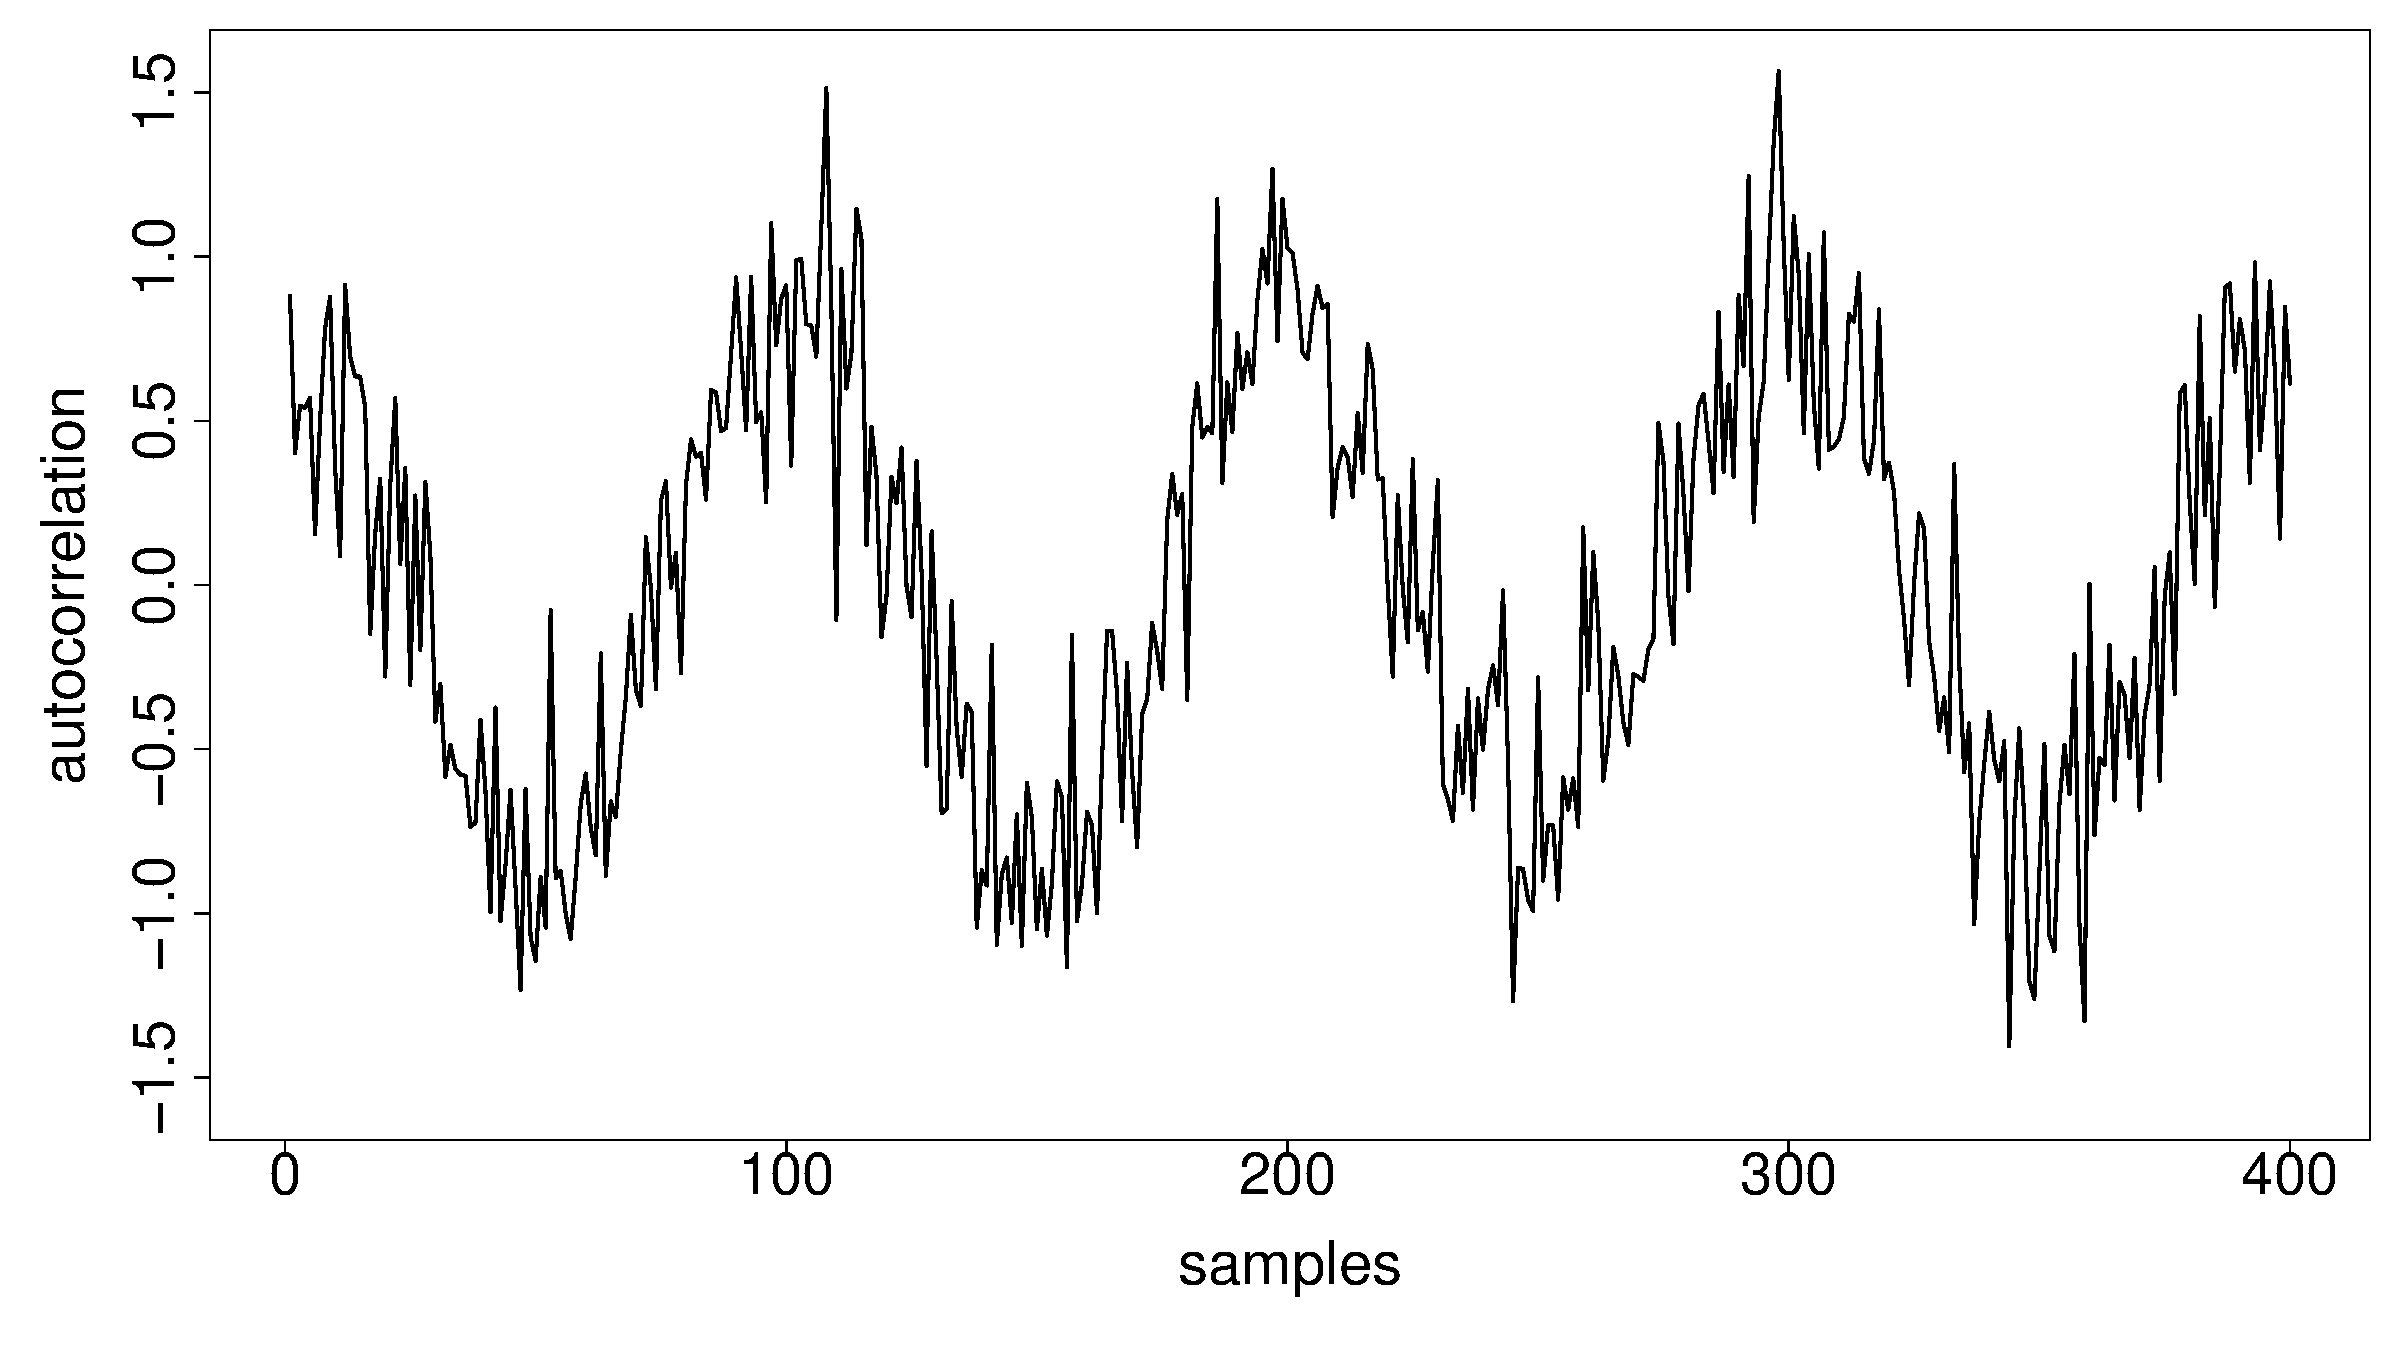
\includegraphics[width=\columnwidth]{figures/autocorrelation}
	\caption{Autocorrelation function of the first \num{400} points of the sample. It is easy to notice the underlying a cosine function.}
	\label{fig:autocorrelation}
\end{figure}

\cref{fig:autocorrelation} shows the autocorrelation function of the first \num{400} points of the data set.
As expected, the function has the shape of a cosine function.
The residual noise due to the variances of $Y$ and $Z$.

It is easy to see from the graph that each period of the sinusoid contains about \num{100} samples.
To get the precise number, we use a numerical approach.
We denote with $lag$ half of the period of the sinusoid.
For an interval of our rough estimation of the $lag$ (in this case \num{50}), we compute the average of the absolute value of the peaks (positive and negative) as a function of the lag's guess.
Then, we take the value that maximizes this function as the estimated lag.

\begin{equation*}
    lag = \argmax_{l} \sum_{\tau=1}^{\big\lfloor \frac{N}{2 \cdot l} \big\rfloor} |R(\tau + l)| + |R(\tau + 2 \cdot l)|
\end{equation*}

Now the frequency $f$ can be estimated as:

\begin{equation*}
    \hat{f} = \frac{F}{2 \cdot lag} = \frac{\SI{20}{\kilo\hertz}}{2 \cdot 50} = \SI{200}{\hertz}
\end{equation*}
